 \documentclass[presentation]{beamer}
\usepackage{../oop-slides-pianini}
\setbeamertemplate{bibliography item}[text]
\newcommand{\lessonnr}[0]{06}
\title[OOP08 -- DCVS, GUI e IO]{08 \\ DVCS, parte II \\ Input-Output e Reflection}

\begin{document}

\frame[label=coverpage]{\titlepage}

%====================
%Outline
%====================
\begin{frame}<beamer>
 	\frametitle{Outline}
 	\tableofcontents[]
\end{frame}

\section{Decentralized Version Control Systems}

\subsection{Risolvere i merge conflict}

\fr{Conflicted files}{
	\bl{In generale}{
		Abbiamo visto nell'ultima lezione come sia possibile riunire due flussi di lavoro diversi.
		%
		Abbiamo anche visto che, nel caso in cui due linee di sviluppo abbiano modificato concorrentemente un file nello stesso punto, il merge non è banale da effettuare ma occorre risolvere manualmente un \emph{merge conflict}.
	}
}

\begin{frame}[fragile]{Esempio di conflict file}
	\begin{block}{}
		\tiny
		\begin{verbatim}
public final class HelloWorld {

    private static final String AUTHOR = "Danilo Pianini";

    public static void main(final String[] args) {
<<<<<<< HEAD
        System.out.println("This program is running in a PC with " + procNumber() + " logic processors!");
    }

    public static int procNumber() {
        return Runtime.getRuntime().availableProcessors();
=======
        System.out.println("This program has been realised by " + AUTHOR);
>>>>>>> feature
    }

}
		\end{verbatim}
	\end{block}
\end{frame}

\fr{Risoluzione del conflitto}{
	\iz {
		\item Modifica dei file che confliggono, fino a portarli allo stato desiderato.
		\item Aggiunta dei file alla staging area (con \texttt{git add})
		\item Salvataggio delle modifiche tramite \texttt{git commit}
		\begin{itemize}
			\item Il messaggio di commit di default nel caso di merge viene auto-generato da Git e può essere mantenuto
		\end{itemize}
	}
}

\fr{Errore frequente: bad tracking}{
	Cosa succede, se per errore abbiamo messo in tracking rigenerabili che non avremmo dovuto mettere?
	\bl{Un altro buon motivo per stare attenti a cosa si mette in tracking}{
		\begin{itemize}
		 \item Se abbiamo dei file binari in tracking (ad esempio dei class files che vengono ricompilati ogni volta), ad \textbf{ogni} merge avremo dei conflitti.
		 \item Ci sarà un conflitto per ogni risorsa modificata. Potenzialmente, centinaia ad ogni merge.
		 \item I conflitti su binari sono difficili da risolvere: il file può essere solo ispezionato tramite editor binari, e buona fortuna a capirne il contenuto.
		 \item Di norma si risolve cancellando tutti i file, rigenerandoli, marcando tutti i conflitti come risolti e facendo un commit.
		 \item \alert{\textbf{ESPLODE}} la dimensione del repository
		 \item State attenti a cosa mettete in tracking!
		\end{itemize}
	}
}

\subsection{Lavorare in remoto: clone, fetch, pull, push}

\fr{Decentralizzazione}{
	\bl{Decentralizzazione totale...}{
		Nei DVCS, non esiste un punto centrale che fa repository ``ufficiale'': tutti i repository ricevono l'intera storia ed hanno pari importanza.
		
		Il design dei DVCS è ideale per un mondo P2P
	}
	\bl{... nella realtà della struttura di Internet}{
		Per via della struttura attuale di Internet, della presenza di NAT e simili strutture di rete, il modello client/server è spesso difficile da aggirare.
		%
		È spesso anche sconveniente aggirarlo: tutto sommato, il cloud spesso è utile...
		
		Esistono servizi di hosting che consentono di avere in un punto sempre accessibile dei repository in rete: chi ha bisogno di collaborare non deve preoccuparsi di problematiche di rete diverse da ``andare sul web''.
	}
}

\fr{Clone}{
	\bl{In generale}{
		Occorre un meccanismo che consenta di fare copie di repository esistenti, al fine di cominciare a lavorare su qualcosa di già esistente, o di effettuare copie di sicurezza del proprio lavoro.
	}
	\bl{In Git}{
		\iz{
			\item \texttt{git clone URI localfolder}
		}
		Scarica l'intera storia del repository conservato in \texttt{URI} all'interno di \texttt{localfolder}, che diventa un repository Git. Esempi di \texttt{URI}:
		\iz {
			\scriptsize
			\item \texttt{/home/user/repository/} --- URI locale (*nix)
			\item \texttt{C:\textbackslash{}Users\textbackslash{}Username\textbackslash{}repository\textbackslash{}} --- URI locale (Windows)
			\item \texttt{ssh://username@server/repository/} --- URI Secure Shell (raccomandata per chi lavora in remoto con server e/o client Unix)
			\item \texttt{https://user@server/repository/} --- URI HTTPS, multipiattaforma
		}
	}
}

\begin{frame}[fragile, allowframebreaks]{Remote repositories}
	\bl{In generale}{
		Vogliamo conservare un riferimento agli URI ai quale si trovano i repository dai quali vogliamo leggere o sui quali vogliamo scrivere.

		In caso di operazioni remote, infatti, è comodo avere un nome simbolico invece di specificare sempre una URI.
	}
	\bl{In Git}{
		Il sottocomando \texttt{git remote} consente di gestire repository remoti. Ogni repository remoto ha un nome ed una URL.
		\begin{itemize}
			\item \texttt{git remote -v}
			\begin{itemize}
				\item Elenca i repository remoti configurati
			\end{itemize}
			\item \texttt{git remote add name url}
			\begin{itemize}
				\item Aggiunge un nuovo repository remoto di nome \texttt{name} che punta ad \texttt{uri}
			\end{itemize}
			\item \texttt{git remote rm name}
			\begin{itemize}
				\item Rimuove il repository remoto \texttt{name}
			\end{itemize}
		\end{itemize}
	}
	\begin{block}{Branch upstream}
		È possibile configurare, per ciascun branch, un uri di un repository remoto dove si andrà a leggere e scrivere a meno di diversa specifica
		\begin{itemize}
			\item Si usa l'opzione \texttt{-u} (\texttt{--set-upstream-to})
			\begin{itemize}
				\item \texttt{git branch -u remoteName/remoteBranch}
				\item D'ora in poi, tutte le operazioni accesso remoto lanciate dal branch corrente verranno mappate sul branch \texttt{remoteBranch} del repository remoto \texttt{remoteName}
			\end{itemize}
		\end{itemize}
		Nel caso in cui il repository sia stato clonato e non inizializzato (ossia, il primo comando dato è stato \texttt{git clone} e non \texttt{git init}), un riferimento al repository di origine viene automaticamente inserito fra i remote e configurato come upstream per tutti i branch col nome di \texttt{origin}.
	\end{block}
	\begin{block}{Visualizzazione dei branch remoti}
		Al momento del clone, Git scaricherà solo il branch ``primario'' (normalmente, \texttt{master}). È possibile comunque visualizzare tutti i branch disponibili in remoto:
		\begin{itemize}
			\item \texttt{git branch -a}
			\begin{itemize}
				\item Elenca tutti i branch, inclusi quelli remoti.
			\end{itemize}
		\end{itemize}
	\end{block}
	\begin{block}{Importazione di branch remoti}
		Qualora si voglia importare in locale un branch remoto per lavorarci, occorre creare un ``tracking branch'' locale:
		\begin{itemize}
			\item \texttt{git checkout -b localBranchName remoteName/remoteBranchName}
			\begin{itemize}
				\item Crea un nuovo branch di nome \texttt{localBranchName}, che avrà i contenuti di \texttt{remoteName/remoteBranchName}
				\item Sovente si dà al branch locale lo stesso nome del branch remoto
				\begin{itemize}
					\item \texttt{git checkout -b develop origin/develop}
				\end{itemize}
			\end{itemize}
		\end{itemize}
	\end{block}
\end{frame}

\begin{frame}[fragile, allowframebreaks]{Fetch e pull}
	\bl{In generale}{
		Vogliamo una operazione che ci consenta di acquisire nuovi commit da una fonte, in maniera tale da acquisire il lavoro fatto da altri. Tale operazione si chiama fetch, e \emph{teoricamente} è l'unica operazione necessaria a rendere completamente distribuito un DVCS.
	}
	\bl{In Git}{
		Il sottocomando \texttt{fetch} scarica i commit da un repository remoto
		\iz{
			\item \texttt{git fetch URI branchName}
			\begin{itemize}
				\item Scarica da \texttt{URI} tutti i commit del branch \texttt{branchName}
			\end{itemize}
			\item \texttt{git fetch remoteName branchName}
			\begin{itemize}
				\item Scarica dal remote \texttt{remoteName} tutti i commit del branch \texttt{branchName}
			\end{itemize}
			\item \texttt{git fetch}
			\begin{itemize}
				\item Scarica dal remote di default (se presente) tutti i commit
			\end{itemize}
			Dopo la \texttt{fetch}, è necessario utilizzare \texttt{git merge} per unire i commit scaricati al branch corrente\texttt{}.
		}
	}
	\begin{block}{Pull}
		Il sottocomando \texttt{pull} (stessa sintassi di \texttt{fetch}) esegue una \texttt{fetch} seguita da un \texttt{merge}, ed è quindi conveniente da usare nel caso in cui si vogliano eseguire entrambe le operazioni.
		\begin{itemize}
			\item \texttt{git pull URI branchName}
			\begin{itemize}
				\item Scarica da \texttt{URI} tutti i commit del branch \texttt{branchName} e prova a mergerli nel branch corrente
			\end{itemize}
			\item \texttt{git pull remoteName branchName}
			\begin{itemize}
				\item Scarica dal remote \texttt{remoteName} tutti i commit del branch \texttt{branchName} e prova a mergerli nel branch corrente
			\end{itemize}
			\item \texttt{git pull}
			\begin{itemize}
				\item Scarica dal remote di default (se presente) tutti i commit e prova a mergerli nel branch corrente
			\end{itemize}
		\end{itemize}
	\end{block}
\end{frame}


\fr{Esempio con \texttt{clone} e \texttt{pull}}{
  Situazione iniziale \\
  \begin{center}
    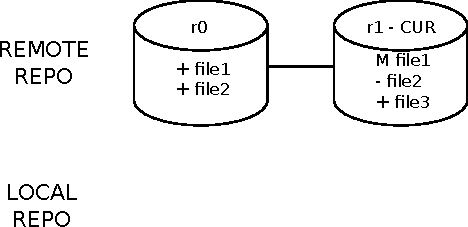
\includegraphics[width=0.99\textwidth]{img/draw3}
  \end{center}
}

\fr{Esempio con \texttt{clone} e \texttt{pull}}{
  Local esegue:\\
  \texttt{git clone indirizzo\_di\_remote\_repo percorso\_di\_local\_repo} \\
  \begin{center}
    \includegraphics[width=0.8\textwidth]{img/draw4}
  \end{center}
}

\fr{Esempio con \texttt{clone} e \texttt{pull}}{
  Local esegue:\\
  modifica di \texttt{file3} \\
  \texttt{commit} \\
  \begin{center}
    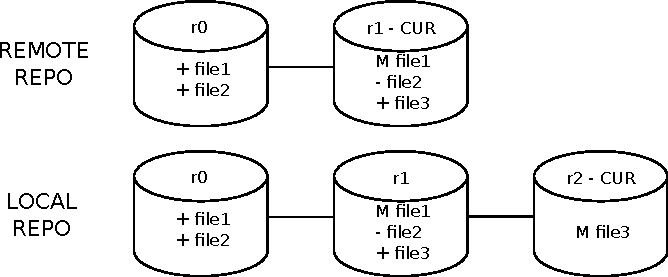
\includegraphics[width=0.99\textwidth]{img/draw5}
  \end{center}
}

\fr{Esempio con \texttt{clone} e \texttt{pull}}{
  Remote esegue:\\
  \texttt{git pull indirizzo\_di\_local\_repo} \\
  \begin{center}
    \includegraphics[width=0.99\textwidth]{img/draw6}
  \end{center}
}

\begin{frame}[fragile, allowframebreaks]
	\bl{In generale}{
		Nella realtà dei fatti le operazione di \texttt{fetch} e \texttt{pull} non sono sufficienti. L'operazione duale della \texttt{pull} si chiama \texttt{push}, ed è più delicata: chi la esegue deve avere i diritti di scrittura verso la destinazione.
	}
	\bl{In Git}{
		\begin{itemize}
			\item \texttt{git push URI branchName}
			\begin{itemize}
				\item Carica sul branch \texttt{branchName} \texttt{URI} tutti i commit del branch 
			\end{itemize}
			\item \texttt{git push remoteName branchName}
			\begin{itemize}
				\item Carica sul remote \texttt{remoteName} tutti i commit del branch \texttt{branchName}
			\end{itemize}
			\item \texttt{git push}
			\begin{itemize}
				\item Carica dal remote di default (se presente) tutti i commit del branch corrente
			\end{itemize}
		\end{itemize}
		Nel caso in cui ci fossero commit sul branch destinazione del repository remoto non presenti in quello locale, la \texttt{push} \textbf{fallirebbe}.
		In questo caso, infatti, è necessario effettuare prima una pull
	}
\end{frame}

\begin{frame}[fragile, allowframebreaks]{Esempio con \texttt{push}}
	Situazione iniziale:
	\begin{center}
		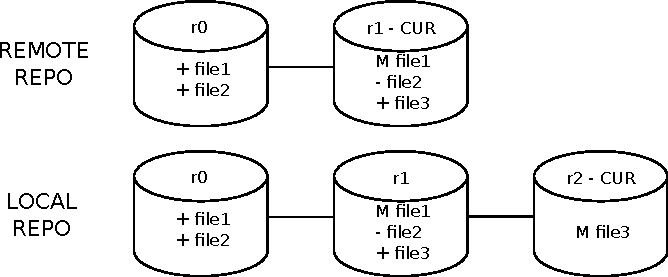
\includegraphics[width=0.99\textwidth]{img/draw5}
	\end{center}
	\framebreak{}
	Local esegue: \texttt{git push indirizzo\_di\_remote\_repo}
	\begin{center}
		\includegraphics[width=0.99\textwidth]{img/draw6}
	\end{center}
\end{frame}

\begin{frame}[fragile, allowframebreaks]{Lavorare in parallelo: esempio}
	Situazione iniziale:
	\begin{center}
		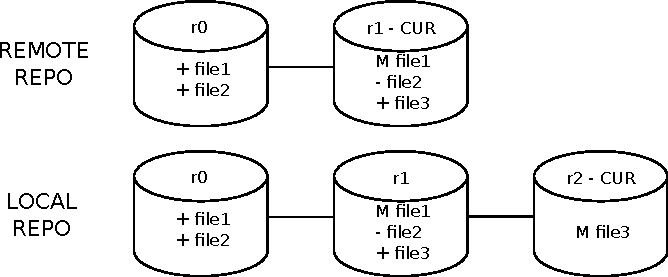
\includegraphics[width=0.99\textwidth]{img/draw5}
	\end{center}
	\framebreak{}
	
	Local esegue: \texttt{git push indirizzo\_di\_remote\_repo}
	\begin{center}
		\includegraphics[width=0.99\textwidth]{img/draw6}
	\end{center}
	\framebreak{}
	
	Remote esegue:\\
	Modifica di \texttt{file2} \\
	\texttt{git commit} \\
	\begin{center}
		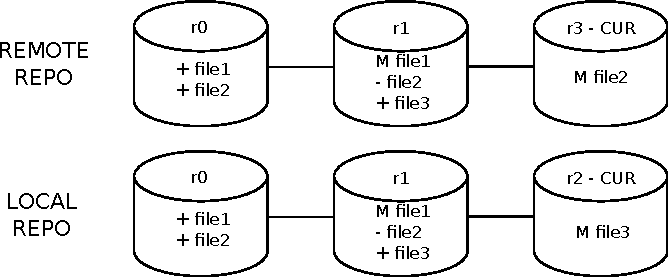
\includegraphics[width=0.99\textwidth]{img/draw7}
	\end{center}
	\framebreak{}
	
	Local esegue:\\
	\texttt{git push indirizzo\_di\_remote\_repo} \\
	\begin{center}
		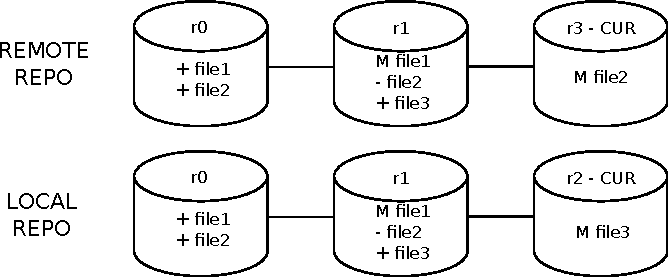
\includegraphics[width=0.99\textwidth]{img/draw7}
	\end{center}
	La push viene rifiutata: la radice dei due repository è diversa!
	\framebreak{}
	
	Local esegue:\\
	\texttt{git pull indirizzo\_di\_remote\_repo} \\
	\begin{center}
		\includegraphics[width=0.99\textwidth]{img/draw9}
	\end{center}
	Ora è possibile effettuare la \texttt{push}!
	\framebreak{}
	
	Local esegue:\\
	\texttt{hg push indirizzo\_di\_remote\_repo} \\
	\begin{center}
		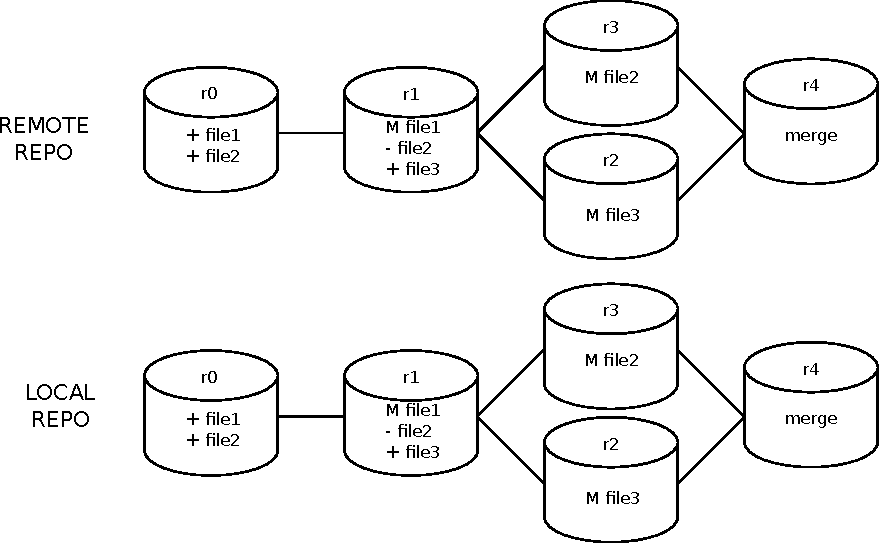
\includegraphics[width=0.8\textwidth]{img/draw10}
	\end{center}
\end{frame}

\subsection{Hosting e Bitbucket}

\fr{Bitbucket Overview}{
	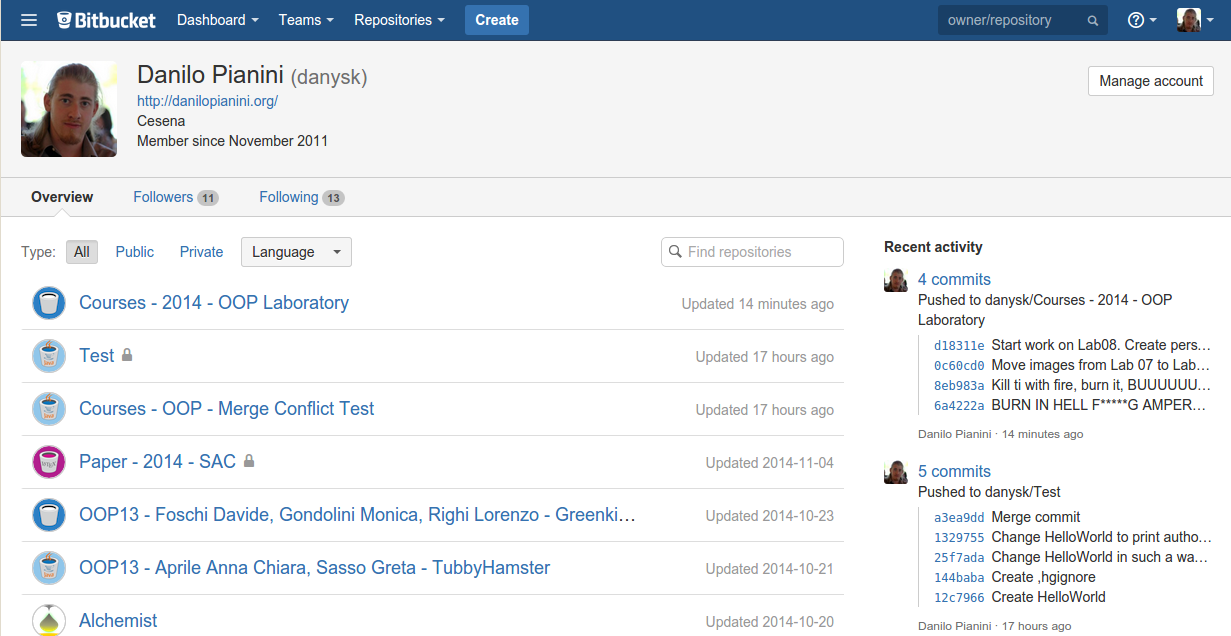
\includegraphics[width=0.99\textwidth]{img/bitbucket0}
}

\fr{Bitbucket Overview}{
	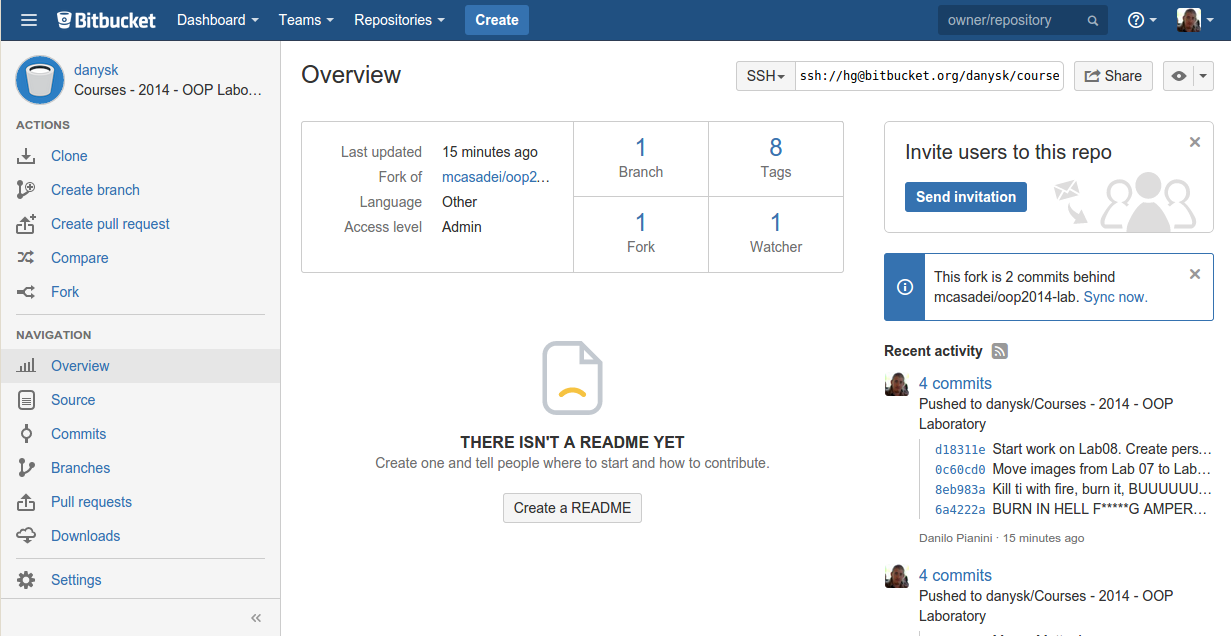
\includegraphics[width=0.99\textwidth]{img/bitbucket1}
}

\fr{Bitbucket Overview}{
	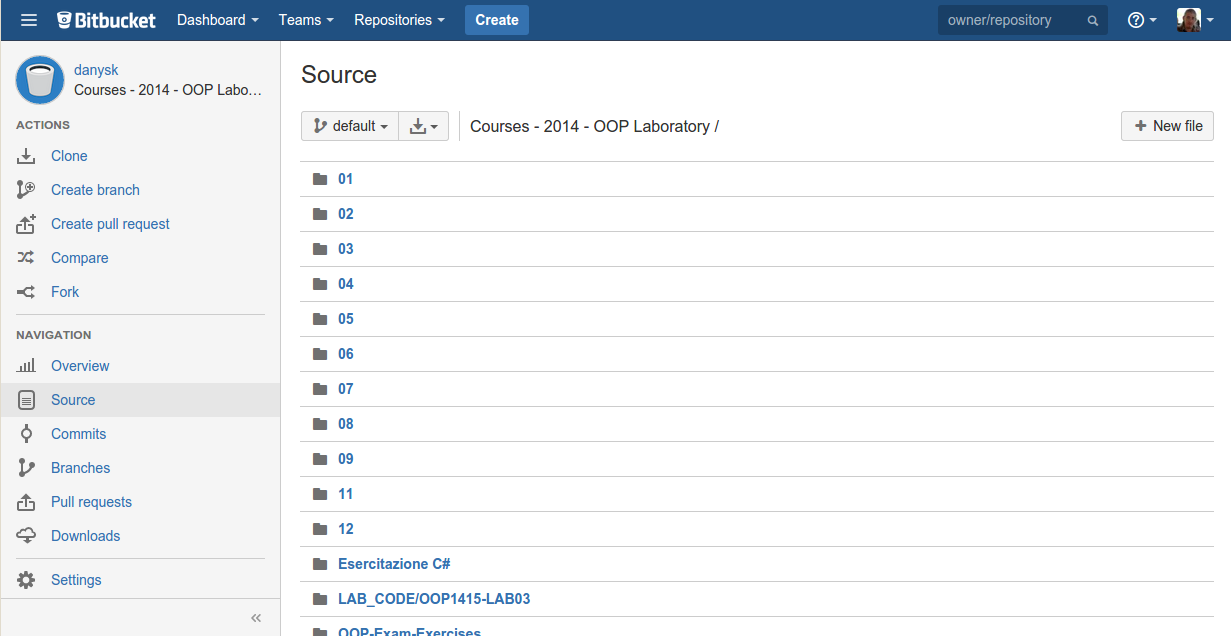
\includegraphics[width=0.99\textwidth]{img/bitbucket2}
}

\fr{Bitbucket Overview}{
	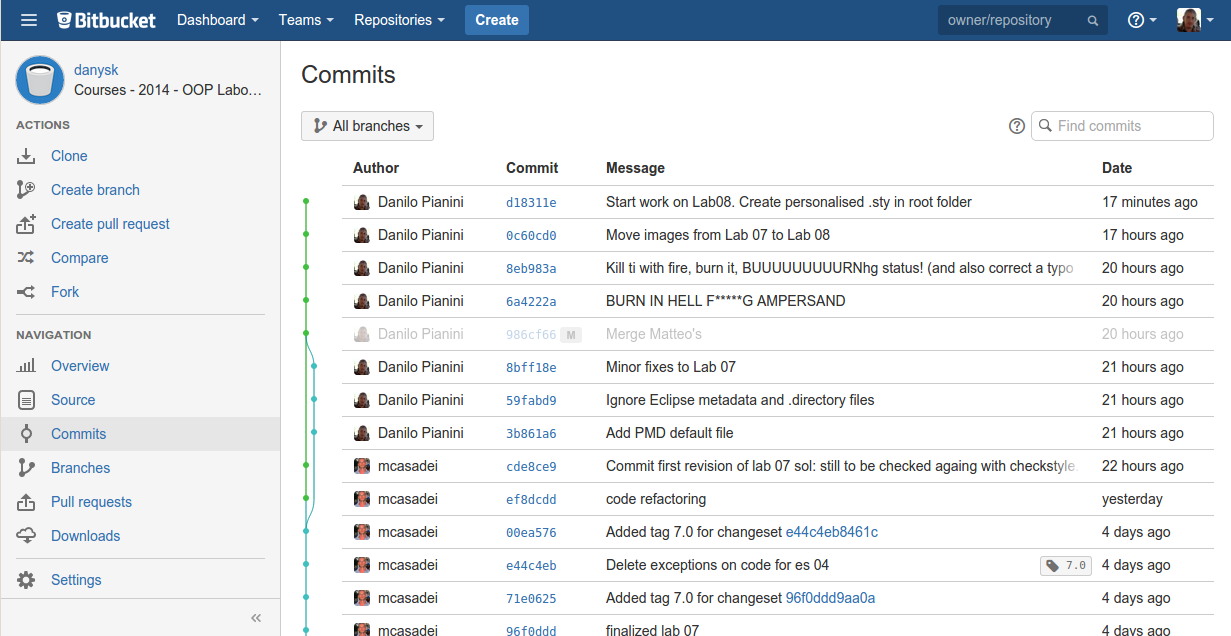
\includegraphics[width=0.99\textwidth]{img/bitbucket3}
}

\fr{Bitbucket Overview}{
	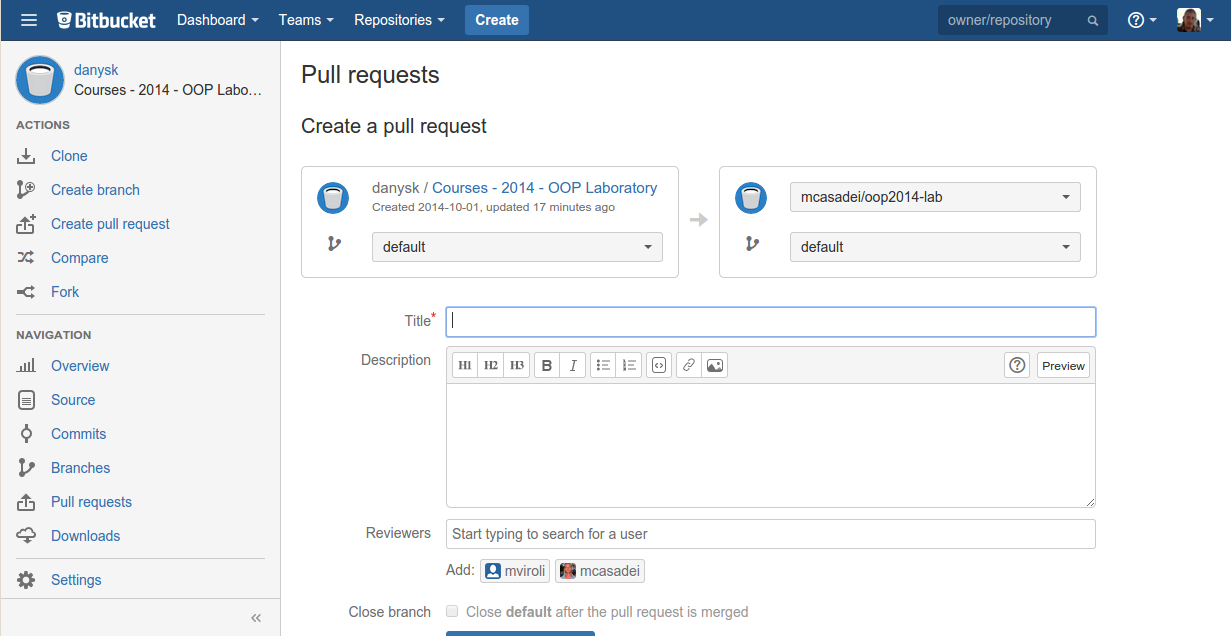
\includegraphics[width=0.99\textwidth]{img/bitbucket4}
}

\fr{Bitbucket Overview}{
	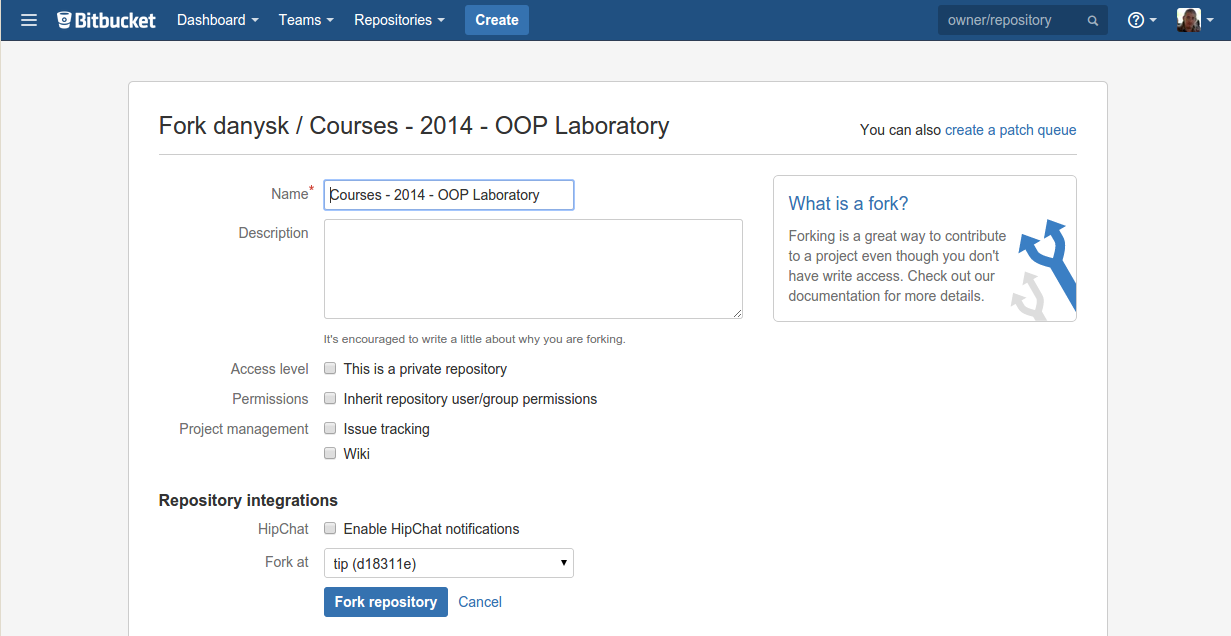
\includegraphics[width=0.99\textwidth]{img/bitbucket5}
}

\fr{Bitbucket Overview}{
	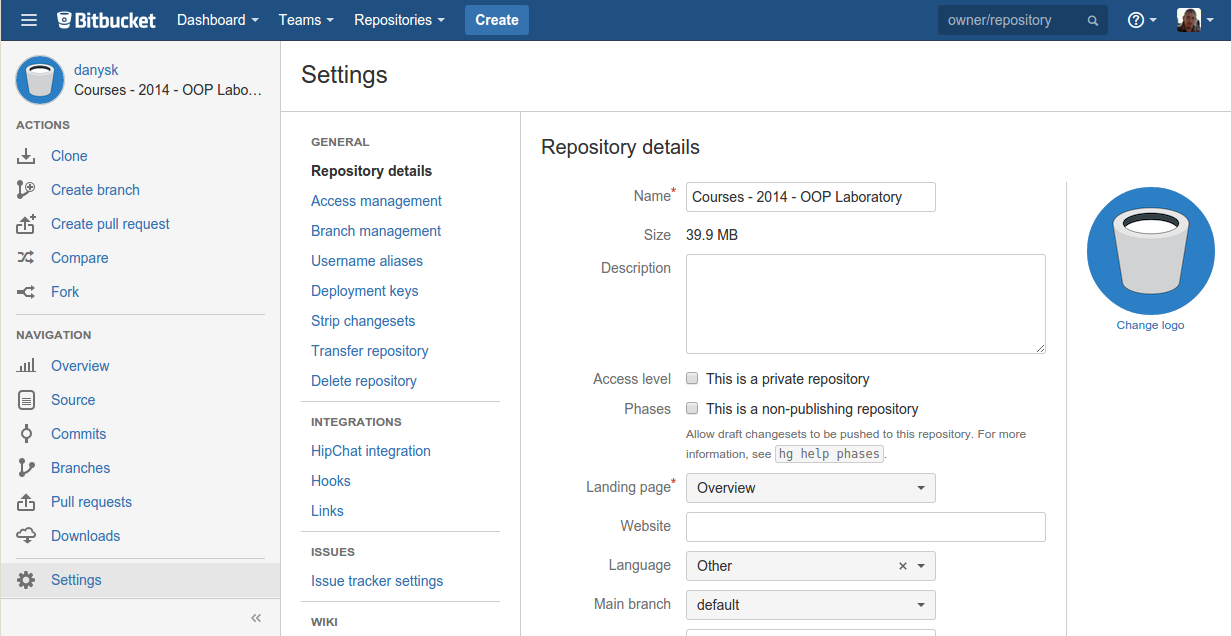
\includegraphics[width=0.99\textwidth]{img/bitbucket6}
}

\fr{Bitbucket Overview}{
	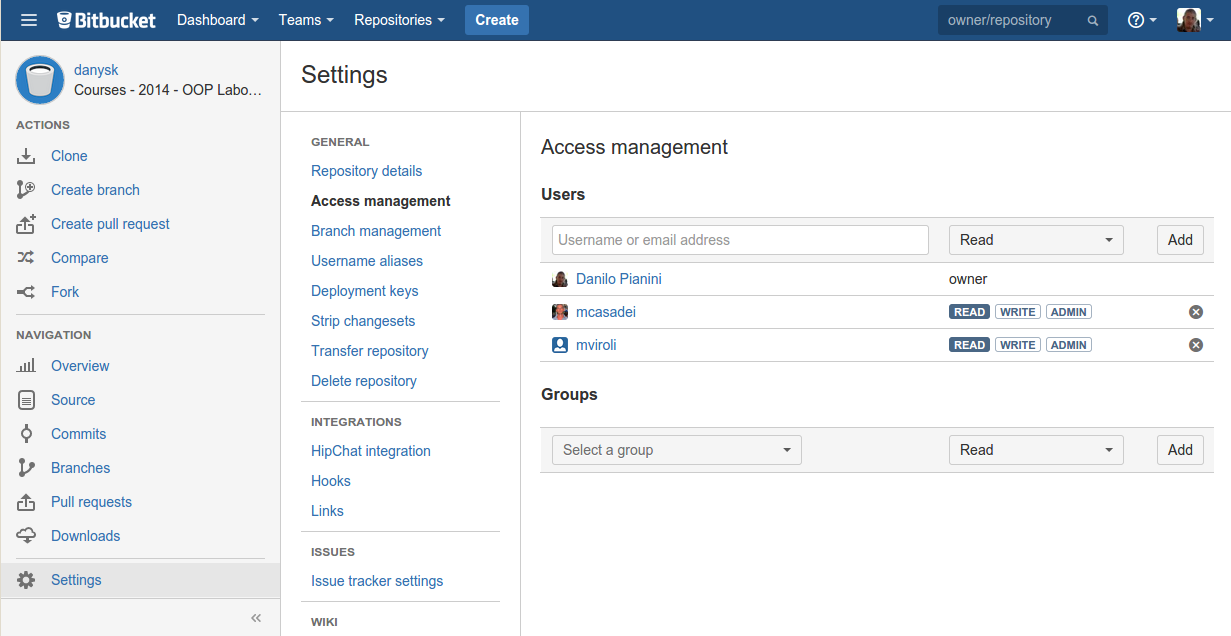
\includegraphics[width=0.99\textwidth]{img/bitbucket7}
}

\fr{Bitbucket Overview}{
	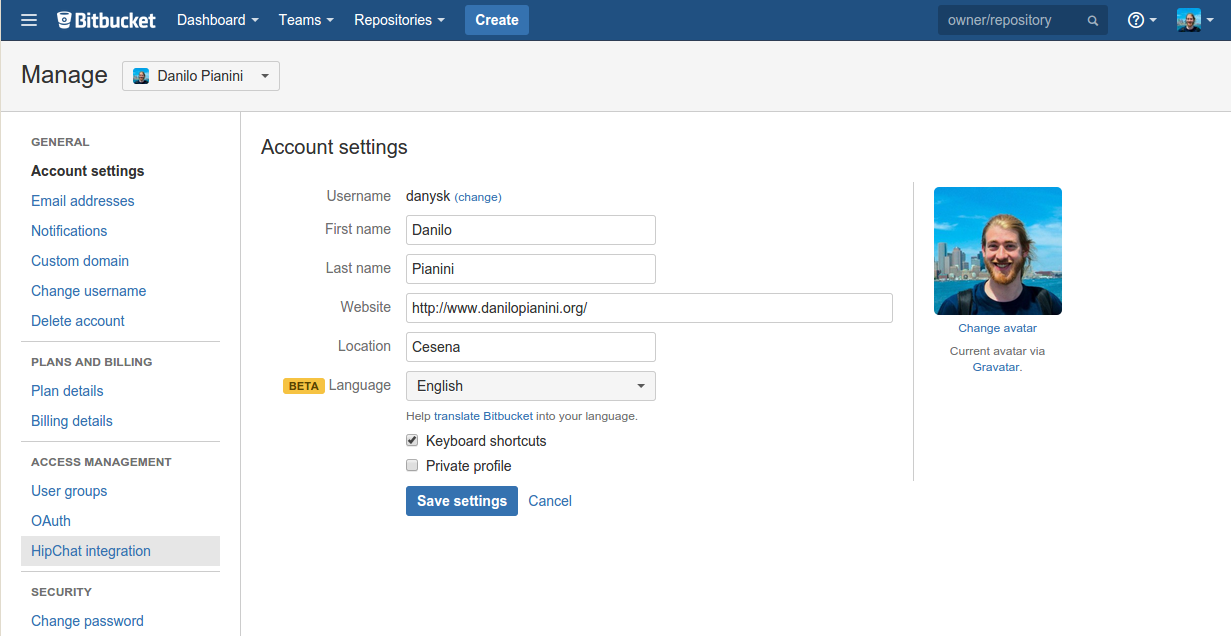
\includegraphics[width=0.99\textwidth]{img/bitbucket9}
}

\fr{Bitbucket Overview}{
	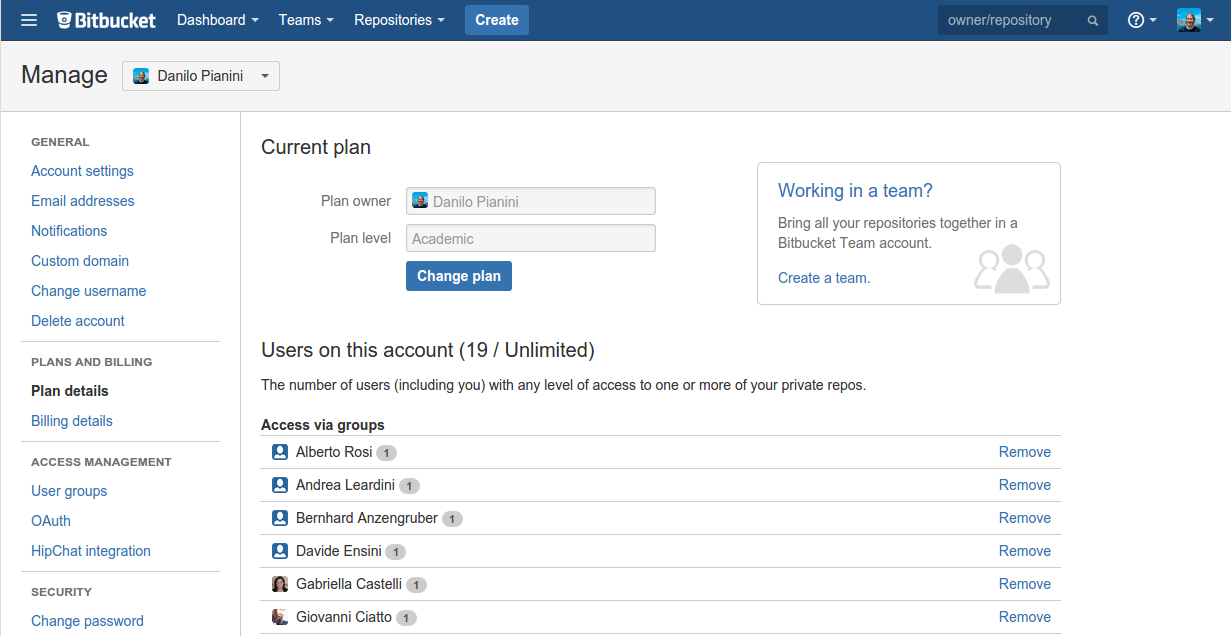
\includegraphics[width=0.99\textwidth]{img/bitbucket10}
}

\fr{Bitbucket Overview}{
	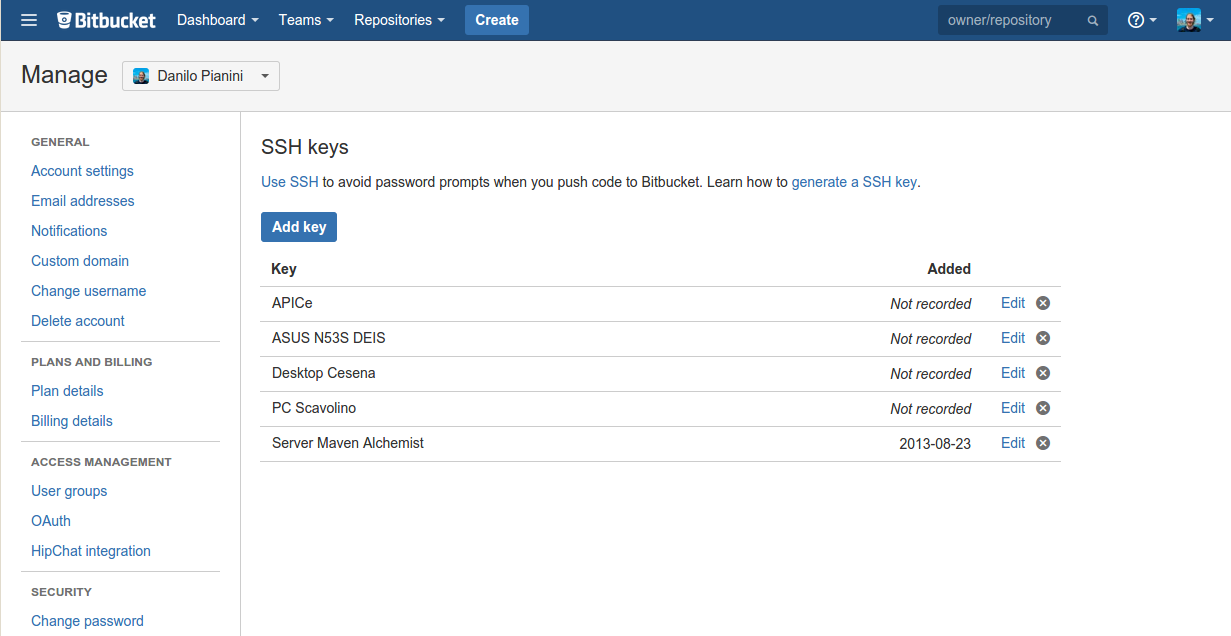
\includegraphics[width=0.99\textwidth]{img/bitbucket11}
}

\fr{Bitbucket Overview}{
	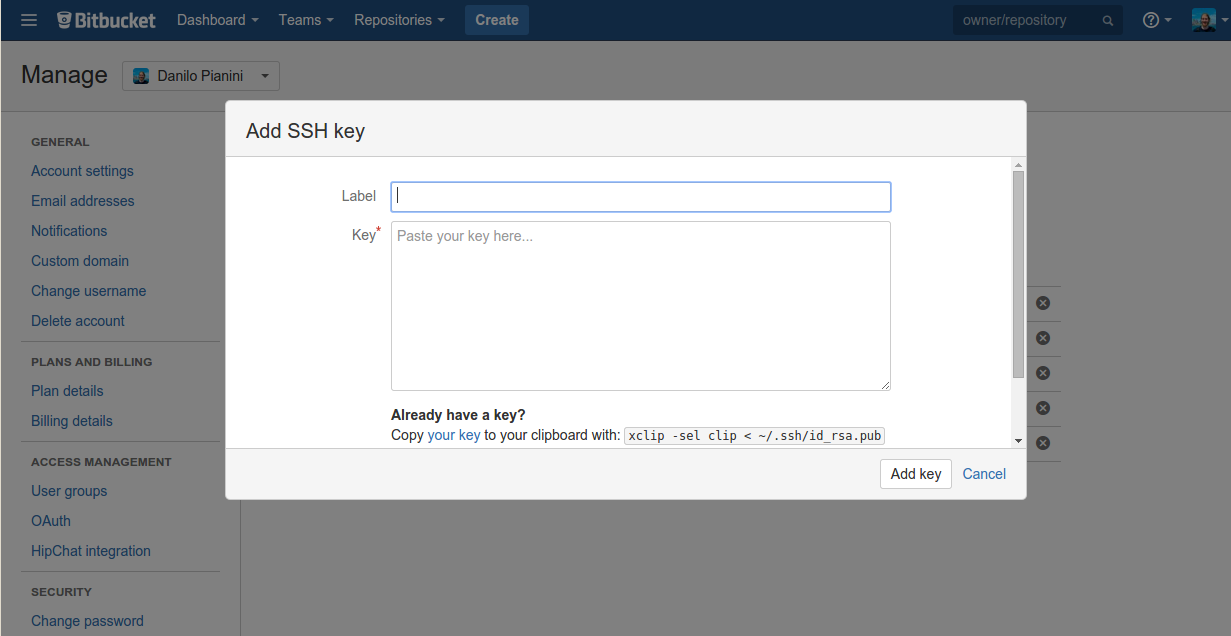
\includegraphics[width=0.99\textwidth]{img/bitbucket12}
	
	\scriptsize
	Su sistemi *nix, si utilizzi il comando \texttt{ssh-keygen -t rsa} per generare una coppia di chiavi pubblica e privata. Non si inserisca alcuna password e si mantengano le opzioni suggerite dal sistema. A questo punto, all'interno della cartella \texttt{\textasciitilde{}/.ssh/}, si troveranno i file delle chiavi. Si incolli nel campo key il contenuto del file \texttt{\textasciitilde{}/.ssh/id\_rsa.pub}

}

\subsection{Plugin Eclipse (eGit)}

\fr{Plugin eclipse}{
	\bl{Installazione}{
		Il plugin è preinstallato dentro la distribuzione di Eclipse.
	}
	\bl{Funzionalità}{
		Il plugin mostrerà le proprie funzionalità dal menu ``Team'', ed esporrà le stesse funzionalità del tool a linea di comando, \alert{mostrando anche quelle che non abbiamo trattato, e che non dovete utilizzare se non avete \textbf{cristallino} il loro funzionamento da terminale}.

		Appare anche una nuova opzione per l'import di un progetto tramite clone di un repository Git.
	}
	È bene (come per tutte le utility con interfaccia grafica) fare un utilizzo \textbf{consapevole} del plugin Eclipse.
	
	Vi consigliamo di preferire l'uso di Git da terminale!
}

\subsection{Features avanzate e prossimo episodio}

\fr{Aspetti avanzati (cenni)}{
  \bl{Rebasing}{
    Procedura alternativa al merge, in cui i due commit, invece di essere fusi, vengono messi in sequenza. Simula una storia ``lineare'' anche dove è in realtà parallela.
  }
  \bl{Cherry picking}{
    Pull di un singolo commit o di un piccolo gruppo di commit. Spesso utilizzato quando si desidera avere un bugfix che si trova in un altro branch, ma non tutto il resto. Molto comune nel backporting delle patch di sicurezza.
  }
  \bl{Bisection}{
    Strategia per scoprire bug in maniera automatizzata, testando il software a varie versioni (ricerca dicotomica). Una volta trovata la prima versione dove il bug si verifica, si controllano commit message e le differenze.
  }
}

\begin{frame}{Nel prossimo episodio}
	\begin{itemize}
		\item Abbiamo in mano uno strumento formidabile per la gestione di progetti
		\item Non ci resta che trovare una strategia efficace per massimizzarne l'efficacia
		\item Vedremo una strategia di lavoro che promuoverà e faciliterà il lavoro in parallelo
	\end{itemize}
\end{frame}


\end{document}

\subsection{Workflow}

\fr{Shared repository}{
  \iz {
    \item Funziona bene se:
    \iz {
      \item Il progetto è piccolo
      \item Ci sono pochi membri nel team
      \item I membri del team possono interagire con facilità
      \item Non c'è un maintainer/leader vero e proprio
    }
    \item Come funziona:
    \iz {
      \item Un solo repository online ``di riferimento''
      \item Tutti i membri fanno pull e push su quello
    }
    \item Regole per farlo funzionare bene:
    \iz {
      \item Ciascun membro deve fare pull prima di fare push
      \item Nel caso in cui la pull richieda di eseguire un'operazione di merge, è responsabilità di chi ha fatto la pull eseguire il merge correttamente prima di fare push
    }
    \item Difetti:
    \iz {
      \item Un solo membro che lavora male può compromettere il repository
      \item Gara a chi fa push per primo per evitare di dover eseguire i merge
    }
  }
}

\fr{Shared repository}{
  \begin{center}
    \includegraphics[width=0.99\textwidth]{img/shared}
  \end{center}
}

\fr{Multiple forks and pull requests}{
  \iz {
    \item Funziona bene se:
    \iz {
      \item Il progetto è grande
      \item I membri del team non riescono a tenersi in contatto, ad esempio perché non lavorano nello stesso ufficio
      \item C'è un maintainer o un responsabile
    }
    \item Come funziona:
    \iz {
      \item Un repository online ``di riferimento'', gestito dal maintainer
      \item Ogni sviluppatore fa una fork del repository principale
      \item Gli sviluppatori pull-ano dal repository principale e push-ano sulla loro fork
      \item Quando la funzionalità che si voleva integrare è pronta per la consegna, lo sviluppatore apre una pull request verso il main repo
      \item Il maintainer può analizzare il codice che verrebbe modificato, se accetta le modifiche il main repo viene portato nello stesso stato della fork.
    }
    \item Regole per farlo funzionare bene:
    \iz {
      \item Il maintainer deve essere in grado di effettuare code review
    }
    \item Difetti:
    \iz {
      \item Più complicato di un singolo repository condiviso
    }
  }
}

\fr{Multiple forks and pull requests}{
  \begin{center}
    \includegraphics[width=0.99\textwidth]{img/forks}
  \end{center}
}



\fr{Esercizio con Mercurial} {
	\iz{
		\item Si acceda a \url{https://bitbucket.org/}
		\item Ci si logghi con il proprio utente
		\item Si vada al progetto che si trova alla pagina \url{https://bitbucket.org/danysk/courses-oop-merge-conflict-test}
		\item Dall'interfaccia web di Bitbucket, si crei una propria fork del progetto
		\item Utilizzando il comando \texttt{hg clone}, si cloni \textbf{la propria fork del progetto} all'interno di una nuova directory
		\item Utilizzando il comando \texttt{hg heads}, si verifichi che il progetto ha due teste
		\item Si tenti di fare il merge utilizzando \texttt{hg merge} 
		\item Si osservi l'output di Mercurial: il merge ha generato un conflitto
		\item Si utilizzi il comando \texttt{ls -ahl} (su Windows si usi l'equivalente \texttt{dir}) per vedere l'elenco dei file
		\item Si noti che è stato creato un file \texttt{.origin}
	}
}

\fr{Esercizio con Mercurial} {
	\iz{
		\item Utilizzando il comando \texttt{cat} (in Windows si usi il comando equivalente \texttt{type}) si osservi il contenuto dei file \texttt{HelloWorld.java.orig} e \texttt{HelloWorld.java}
		\item Si modifichi HelloWorld.java in modo che stampi le informazioni riguardanti l'autore (non si modifichi l'autore al momento) e che stampi nella linea successiva l'informazione sul numero di processori installati.
		\item Si compili nella cartella \texttt{bin} il file \texttt{HelloWorld.java}
		\item Se ne testi il funzionamento
		\item Una volta che il programma è funzionante, si usi hg status per vedere lo stato del repository. Si noti che il file \texttt{.orig} è in stato \texttt{?}
		\item Si elimini il file \texttt{.orig}
		\item Si dichiari risolto il conflitto di merge di \texttt{HelloWorld.java} utilizzando propriamente il comando \texttt{hg resolve -m}
		\item Si salvi il merge con \texttt{hg commit}
	}
}

\fr{Esercizio con Mercurial} {
	\iz{
		\item Dall'interfaccia web di Bitbucket, si crei un nuovo repository online
		\item Si faccia \texttt{hg push} del repository locale verso il nuovo repository online
		\item Si osservi, nell'interfaccia web di Bitbucket, la storia dei commit ed il grafo che mostra l'evoluzione dei flussi di lavoro
		\item Si modifichi \texttt{HelloWorld.java} in modo tale che stampi il nome e cognome dello studente
		\item Si esegua commit
		\item In una nuova cartella \textbf{fuori dal repository corrente}, si cloni la precedente fork del repository (che avrà ancora le due teste separate)
		\item Si modifichi il file \texttt{.hg/hgrc} facendo sì che punti al nuovo repository creato su Bitbucket
		\item Si eseguano \texttt{hg pull} e \texttt{hg update}
		\item Si verifichi con \texttt{hg log} e \texttt{hg heads} che il nuovo repository locale ha incorporato le modifiche fatte in precedenza. 
	}
}


